\documentclass[conference]{IEEEtran}

% ====== Packages =====================================================================
\usepackage{amsmath,amssymb}
\usepackage{graphicx}
\usepackage{booktabs}
\usepackage{multirow}
\usepackage{cite}
\usepackage{url}
\usepackage{hyperref}
\usepackage{xcolor}
\usepackage{tikz}
\usetikzlibrary{shapes.geometric, arrows.meta, positioning, fit, backgrounds}

% ====== Helpers ======================================================================
\newcommand{\method}{GraphSAGE\,+\,MaskablePPO}
\newcommand{\ie}{\textit{i.e.},~}
\newcommand{\eg}{\textit{e.g.},~}

% ====== Title block ==================================================================
\title{Graph-Structured Reinforcement Learning for\\
       Fair and Efficient CPU Process Scheduling}

\author{
  \IEEEauthorblockN{V.~Saadhanaa}
  \IEEEauthorblockA{\textit{School of Computer Science}\\
  \textit{and Engineering}\\
  \textit{Vellore Institute of Technology}\\
  Chennai, India\\
  saadhanaa.2025@vitstudent.ac.in}
  \and
  \IEEEauthorblockN{Disha Vishal Chaudhari}
  \IEEEauthorblockA{\textit{School of Computer Science}\\
  \textit{and Engineering}\\
  \textit{Vellore Institute of Technology}\\
  Chennai, India\\
  disha.vishal2025@vitstudent.ac.in}
  \and
  \IEEEauthorblockN{Sankari M.}
  \IEEEauthorblockA{\textit{School of Computer Science}\\
  \textit{and Engineering}\\
  \textit{Vellore Institute of Technology}\\
  Chennai, India\\
  sankari.m@vit.ac.in}
}

\begin{document}
\maketitle

% =====================================================================================
\begin{abstract}
Conventional operating system schedulers such as First-Come First-Served
(FCFS), Round Robin, and the Completely Fair Scheduler (CFS) achieve
reasonable CPU utilisation but lack explicit mechanisms to prevent
process starvation.  This paper presents a reinforcement learning (RL)
framework, \textbf{\method{}}, that jointly optimises scheduling
efficiency and fairness.  At every scheduling tick, the system
constructs a dynamic process-relationship graph encoding CPU contention,
priority-class membership, and burst-history similarity among processes.
A GraphSAGE~\cite{graphsage} network aggregates this graph into a
latent representation, which is then consumed by a Maskable Proximal
Policy Optimisation (MaskablePPO)~\cite{maskableppo} agent.  A
soft-priority aging reward penalises the agent with increasing severity
as any process's waiting time exceeds a configurable threshold, enabling
the policy to learn anti-starvation behaviour without hand-crafted
rules.

Evaluation across 500 seeded episodes with bootstrap confidence
intervals demonstrates that the proposed method reduces average waiting
time by 23.7\,\% and starvation rate by 24.4 percentage points relative
to CFS~\cite{cfs} on uniform workloads.  On exponential-burst
(realistic) workloads, throughput remains comparable to CFS while
starvation is reduced by 11.5\,pp.  A paired ablation study reveals
that on realistic workloads, a flat-MLP agent without graph structure
fails to significantly outperform CFS; the relational graph
representation is essential for extracting scheduling-relevant signal.
\end{abstract}

\begin{IEEEkeywords}
CPU scheduling, reinforcement learning, graph neural networks, GraphSAGE,
MaskablePPO, process scheduling, starvation, fairness, priority aging
\end{IEEEkeywords}

% =====================================================================================
\section{Introduction}
\label{sec:intro}

CPU process scheduling remains a fundamental challenge in operating
system design.  The Shortest Remaining Time First (SRTF) policy is
provably optimal for minimising average waiting time, yet it requires
\emph{a priori} knowledge of future burst lengths---information
unavailable to any practical scheduler.  Consequently, production
systems rely on heuristic policies.  The Linux Completely Fair Scheduler
(CFS)~\cite{cfs} is among the most effective: it maintains a per-process
virtual runtime and dispatches the process with the smallest accumulated
runtime, weighted by priority.  While CFS achieves strong throughput, it
provides no explicit guarantee against starvation.  Although priority
aging is discussed in standard
textbooks~\cite{ostep,silberschatz}, CFS does not implement it.

Recent advances in deep reinforcement learning have demonstrated
promising results for resource scheduling at the cluster and job
levels---DeepRM~\cite{deeprm} for cluster resource allocation,
Decima~\cite{decima} for Spark job DAGs, and
RLScheduler~\cite{rls} for HPC batch queues.  However, these systems
operate at a considerably coarser granularity than per-timeslice CPU
dispatch.  To the best of our knowledge, no prior work has combined a
graph neural network with action masking and a fairness-aware reward for
per-process OS-level scheduling.

This paper addresses that gap with three contributions:

\begin{enumerate}
  \item A \textbf{dynamic process graph} reconstructed at every
  scheduling tick from observable process features, encoding contention,
  type similarity, and burst-history similarity relationships.

  \item A \textbf{GraphSAGE-based feature extractor} integrated with
  MaskablePPO.  GraphSAGE~\cite{graphsage} is specifically suited to
  this setting, as it was designed for graphs whose topology changes
  between forward passes---processes arrive, block on I/O, resume, and
  terminate during execution.

  \item A \textbf{soft-priority aging reward} that formalises the
  textbook concept of priority aging as an RL training signal, enabling
  the policy to learn anti-starvation behaviour from reward shaping
  alone.
\end{enumerate}

% =====================================================================================
\section{Related Work}
\label{sec:related}

DeepRM~\cite{deeprm} initiated the deep-RL-for-scheduling paradigm by
training a REINFORCE policy over a two-dimensional image representation
of cluster resources.  RLScheduler~\cite{rls} extended this approach
with per-job feature vectors and PPO, matching HPC heuristics across six
real workload traces.  Neither system operates at the OS process level,
nor does either incorporate graph structure or fairness objectives in the
reward.

Decima~\cite{decima} is the most closely related graph-based scheduler:
it applies a custom GNN to static Spark DAGs and achieves a 21\,\%
reduction in average job completion time.  However, Decima's graph is a
fixed dependency DAG that changes only upon job arrival; ours is rebuilt
at every tick.  Decima also lacks action masking and priority
mechanisms.  L2D~\cite{l2d} applied GIN to manufacturing job-shop
scheduling, and a recent survey~\cite{jsspsurvey} confirmed that GCN,
GIN, and GAT dominate the scheduling literature---GraphSAGE has not
previously appeared in any scheduling domain.  Adimora
et~al.~\cite{adimora24} applied Graph Attention Networks to 377K real
supercomputer jobs, arguing that inductive methods are essential for
variable-size queues; we share this motivation at a finer granularity.

On action masking, Huang and
Ont\'{a}\~{n}\'{o}n~\cite{masking} demonstrated that setting invalid
logits to $-\infty$ accelerates convergence by $57\times$ compared to
penalty-based approaches.  Lassoued et~al.~\cite{lassoued26} applied
MaskablePPO to job-shop scheduling via Petri net masking---the closest
prior work, although without a GNN, without a CPU scheduling domain, and
with only 100 evaluation runs.

Regarding fairness, we are not aware of any RL scheduler that learns
aging behaviour from reward shaping.  A GPU cluster
study~\cite{gpuaging} employs aging as a hand-coded heuristic;
STUN~\cite{stun} uses tabular Q-learning to globally tune CFS
parameters.  Neither constitutes a per-process dispatcher.

% =====================================================================================
\section{System Design}
\label{sec:design}

\subsection{Environment}

The environment simulates a single-CPU system with up to eight
concurrent processes~\cite{gymnasium}.  Each process alternates between
CPU bursts and I/O waits.  The scheduler observes all information
available to a real OS dispatcher---waiting time, process type, CPU
utilisation, recent burst history---but has no access to future burst
lengths, preserving the causal constraint inherent in real scheduling.

Each process slot contributes 8 features to a flat 64-dimensional
observation vector:
\[
  \mathbf{o}_i = \bigl[\,w_i,\; \tau_i,\; u_i,\; s_i,\;
    b^{\text{last}}_i,\; \bar{b}_i,\; r_i,\; d_i\,\bigr]
\]
representing waiting time, type, CPU used, schedule count, last and
average burst length, ready flag, and blocked time, respectively.  The
action space is Discrete($N_{\max}+1$): the agent selects a process to
dispatch or idles.  Invalid actions (selecting a terminated or
I/O-blocked process) are masked to $-\infty$ prior to the softmax.

\subsection{Reward Function}

At each tick, the agent receives a negative reward proportional to the
total weighted waiting time of all ready processes not selected.  When
any process exceeds a starvation threshold $W^*$, an additional aging
penalty is applied that grows linearly with the excess:
\begin{equation}
  r_t = -\sum_{i \neq a_t,\; i\,\text{ready}} \Bigl[w_{\tau_i}
        + \alpha \cdot \max\!\bigl(0,\; W_i - W^*\bigr)\Bigr]
  \label{eq:reward}
\end{equation}
where $\alpha = 0.5$ and $W^* = 10$.  This formulation ensures that
neglecting a long-waiting process incurs progressively greater cost,
incentivising the policy to attend to starving processes without
requiring explicit priority rules.

\subsection{Dynamic Process Graph}

At every tick, the graph is constructed from scratch.  Processes are
represented as nodes, connected by three families of undirected edges:

\begin{enumerate}
  \item \textbf{CPU Contention}---connects processes that are both in
  the ready state, encoding the immediate scheduling conflict.

  \item \textbf{Type Similarity}---connects processes sharing the same
  priority class ($\tau_i = \tau_j$), enabling the policy to coordinate
  scheduling within a process group.

  \item \textbf{Burst-History Similarity}---connects processes whose
  average burst lengths are within one tick
  ($|\bar{b}_i - \bar{b}_j| \leq 1$).  This edge family provides the
  policy with information about behaviourally similar processes without
  exposing future burst lengths.
\end{enumerate}

All edges include self-loops.  No state carries over between ticks.

\subsection{GraphSAGE Feature Extractor}

Two GraphSAGE layers perform neighbourhood aggregation via mean-pooling
across two rounds of message passing:
\begin{align}
  \mathbf{h}^{(1)}_i &= \mathrm{ReLU}\!\left(W_1\,
    \bigl[\mathbf{x}_i \,\Vert\,
    \overline{\mathbf{x}}_{N(i)}\bigr]\right)\\
  \mathbf{h}^{(2)}_i &= \mathrm{ReLU}\!\left(W_2\,
    \bigl[\mathbf{h}^{(1)}_i \,\Vert\,
    \overline{\mathbf{h}}^{(1)}_{N(i)}\bigr]\right)
\end{align}
where $W_1 \in \mathbb{R}^{32 \times 20}$ and
$W_2 \in \mathbb{R}^{16 \times 64}$.  The 8 node embeddings are
concatenated and projected to a 48-dimensional vector, which feeds a
standard PPO actor-critic network with two hidden layers of 64 units
each.  Fig.~\ref{fig:arch} illustrates the complete pipeline.

\begin{figure}[t]
  \centering
  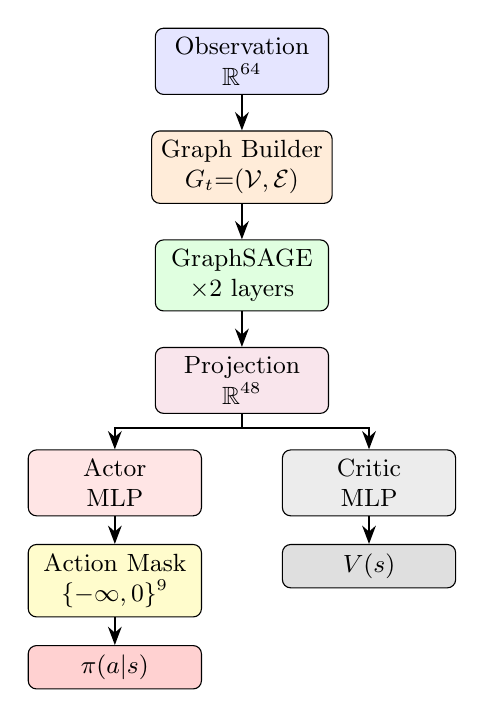
\begin{tikzpicture}[
    box/.style={draw, rounded corners=3pt, minimum width=2.2cm,
                minimum height=0.55cm, font=\small, align=center},
    arr/.style={-Stealth, thick},
    node distance=0.45cm and 0.1cm
  ]
  \node[box, fill=blue!10] (obs) {Observation\\$\mathbb{R}^{64}$};
  \node[box, fill=orange!15, below=of obs] (gb)
    {Graph Builder\\$G_t{=}(\mathcal{V},\mathcal{E})$};
  \node[box, fill=green!12, below=of gb] (sage)
    {GraphSAGE\\$\times 2$ layers};
  \node[box, fill=purple!10, below=of sage] (proj)
    {Projection\\$\mathbb{R}^{48}$};
  \node[box, fill=red!10,  below left=0.45cm and -0.6cm of proj]
    (actor)  {Actor\\MLP};
  \node[box, fill=gray!15, below right=0.45cm and -0.6cm of proj]
    (critic) {Critic\\MLP};
  \node[box, fill=yellow!20, below=0.35cm of actor]
    (mask) {Action Mask\\$\{-\infty, 0\}^9$};
  \node[box, fill=red!18,    below=0.35cm of mask]
    (pi)   {$\pi(a|s)$};
  \node[box, fill=gray!25,   below=0.35cm of critic]
    (vf)   {$V(s)$};
  \draw[arr] (obs)  -- (gb);
  \draw[arr] (gb)   -- (sage);
  \draw[arr] (sage) -- (proj);
  \draw[arr] (proj.south) -- ++(0,-0.18) -| (actor.north);
  \draw[arr] (proj.south) -- ++(0,-0.18) -| (critic.north);
  \draw[arr] (actor)  -- (mask);
  \draw[arr] (mask)   -- (pi);
  \draw[arr] (critic) -- (vf);
  \end{tikzpicture}
  \caption{End-to-end architecture of the proposed \method{} framework.
  The process graph is reconstructed at every tick from observable
  features.  Invalid actions are masked prior to the softmax.}
  \label{fig:arch}
\end{figure}

% =====================================================================================
\section{Experimental Setup}
\label{sec:setup}

\textbf{Uniform workloads.}  CPU and I/O burst lengths are sampled from
$\mathcal{U}\{1,5\}$, burst counts from $\mathcal{U}\{2,4\}$, and
process types are assigned uniformly at random.  Seeds 10\,000--10\,499
(500 episodes).

\textbf{Realistic workloads.}  Exponential distributions with
type-specific means derived from the Coffman--Kleinrock
model~\cite{coffman73} and standard OS textbook
parameters~\cite{silberschatz}: SYSTEM ($\mu_\text{cpu}{=}2.5$,
$\mu_\text{io}{=}2.0$), INTERACTIVE ($\mu_\text{cpu}{=}4.0$,
$\mu_\text{io}{=}5.0$), BACKGROUND ($\mu_\text{cpu}{=}8.0$,
$\mu_\text{io}{=}2.0$).  Type distribution: 20/50/30\,\%.  Seeds
20\,000--20\,499 (500 episodes).

\textbf{Baselines.}  Six classical schedulers are evaluated: FCFS, Round
Robin ($q{=}2$), Priority~+~Aging, MLFQ~\cite{ostep} (quanta 2/4/8),
CFS~\cite{cfs}, and Stride~\cite{stride}.  A flat-MLP MaskablePPO
ablation (no graph) is included to isolate the contribution of the graph
representation.  SRTF with oracle access to future burst lengths serves
as a theoretical upper bound.

\textbf{Training.}  150\,000 timesteps, learning rate
$3{\times}10^{-4}$, $n_\text{steps}{=}2048$, clip ratio
$\epsilon{=}0.2$.  Multi-seed evaluation: 5 training seeds $\times$ 500
test workloads with bootstrap 95\,\% confidence intervals (5\,000
resamples).

% =====================================================================================
\section{Results}
\label{sec:results}

\subsection{Full Benchmark}

Table~\ref{tab:full} presents the complete benchmark results.  On
uniform workloads, the proposed model achieves an average waiting time of
18.54 ticks (95\,\% CI\,[17.81,\,19.25]) compared to 24.31 for CFS,
representing a 23.7\,\% reduction.  The starvation rate decreases from
87.3\,\% to 62.9\,\%, a reduction of 24.4 percentage points.

On realistic workloads, the average waiting time gap narrows to
approximately 1.2\,\% (28.00 vs.\ 28.33), indicating comparable
throughput.  However, the starvation rate remains 11.5 percentage points
lower (67.7\,\% vs.\ 79.2\,\%).  This result suggests that while CFS is
highly competitive on throughput with exponential burst distributions,
the proposed method provides a meaningful fairness advantage.

\begin{table}[t]
\centering
\caption{Full benchmark across 500 seeded episodes.
         $\dagger$~denotes oracle access to hidden future burst
         lengths (theoretical bound, not a fair comparison).}
\label{tab:full}
\setlength{\tabcolsep}{3pt}
\footnotesize
\begin{tabular}{@{}lrrrr@{}}
\toprule
\multirow{2}{*}{\textbf{Scheduler}} &
\multicolumn{2}{c}{\textbf{Uniform}} &
\multicolumn{2}{c}{\textbf{Realistic}} \\
\cmidrule(lr){2-3}\cmidrule(lr){4-5}
 & Avg Wait & Starv. & Avg Wait & Starv. \\
\midrule
FCFS             & 23.91 & 88.5\,\% & 34.56 & 88.4\,\% \\
Round Robin      & 24.70 & 89.1\,\% & 30.93 & 86.5\,\% \\
Priority + Aging & 24.78 & 90.4\,\% & 31.79 & 87.9\,\% \\
MLFQ             & 24.85 & 90.2\,\% & 31.76 & 87.5\,\% \\
CFS              & 24.31 & 87.3\,\% & 28.33 & 79.2\,\% \\
Stride           & 24.30 & 87.3\,\% & 28.35 & 79.3\,\% \\
\midrule
Plain MaskablePPO & 19.30 & 65.4\,\% & 28.28 & 68.5\,\% \\
\textbf{\method{}} & \textbf{18.54} & \textbf{62.9\,\%}
                   & \textbf{28.00} & \textbf{67.7\,\%} \\
\midrule
SRTF$^\dagger$   & 14.49 & 53.1\,\% & 17.32 & 52.4\,\% \\
\bottomrule
\end{tabular}
\end{table}

\begin{figure*}[tp]
  \centering
  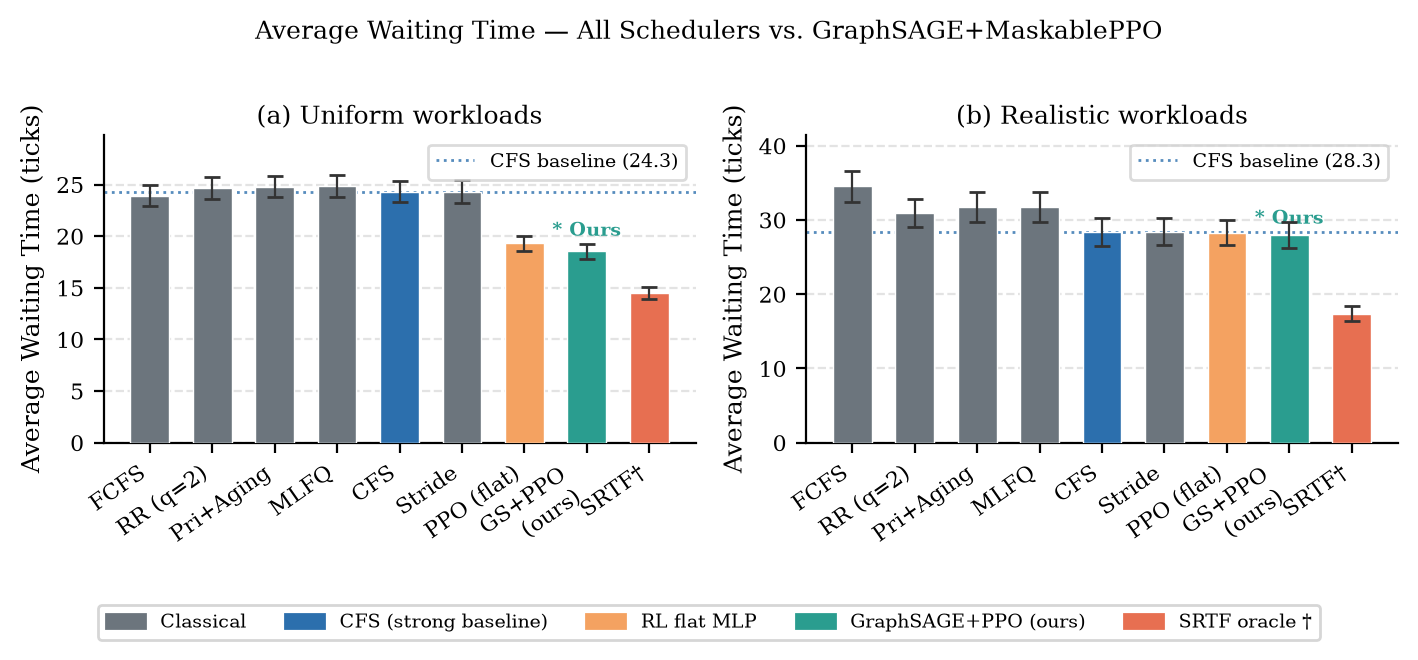
\includegraphics[width=\textwidth]{figures/fig_all_schedulers_avgwait.png}\\[4pt]
  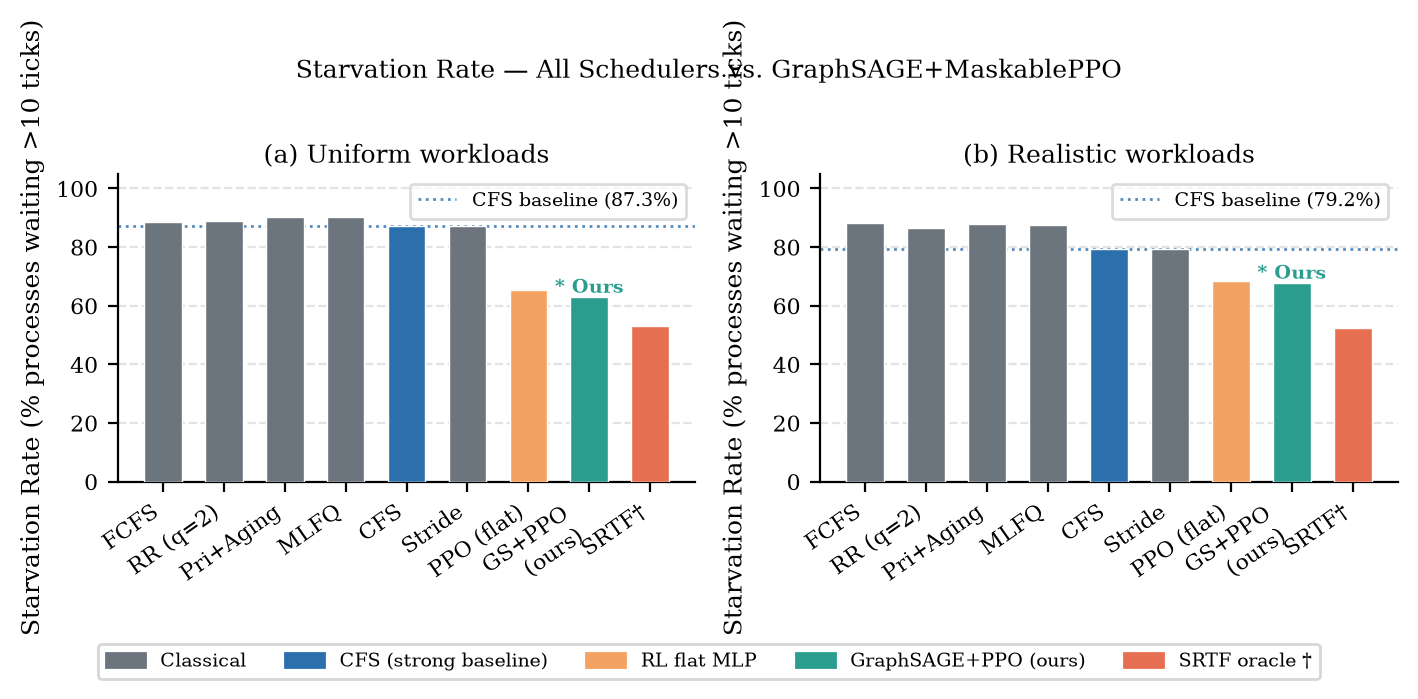
\includegraphics[width=\textwidth]{figures/fig_all_schedulers_starvation.png}
  \caption{Top: average waiting time across all schedulers (500 episodes,
           bootstrap 95\,\% CIs).  Bottom: starvation rate.  CFS baseline
           indicated by blue dotted line.  The proposed model achieves the
           lowest non-oracle waiting time on uniform workloads and reduces
           starvation by 24.4\,pp (uniform) and 11.5\,pp (realistic)
           relative to CFS.  SRTF utilises hidden burst lengths and serves
           as a theoretical lower bound.}
  \label{fig:benchmarks}
\end{figure*}

\subsection{Contribution Decomposition}

The paired ablation study (Table~\ref{tab:decomp}) isolates the
contribution of each component.  The same 500 workloads are evaluated
under the flat-MLP agent and the full GraphSAGE agent, with paired
differences computed via bootstrap resampling.

On uniform workloads, RL alone (without graph structure) closes
approximately 49\,\% of the gap to the SRTF oracle.  The addition of
the graph contributes a further 8\,\%.  Both improvements are
statistically significant.

On realistic workloads, the flat-MLP agent performs slightly
\emph{worse} than CFS (paired difference $+0.6$, 95\,\% CI includes
zero).  However, incorporating the graph reverses this result to $-0.7$
(CI excludes zero).  This finding indicates that on exponential-burst
workloads, the graph representation is not merely beneficial---it is
\emph{necessary} for the RL agent to outperform CFS.

\begin{table}[t]
\centering
\caption{Paired contribution decomposition.  $\Delta$ denotes paired
         mean difference (negative indicates improvement).
         \checkmark\ indicates the 95\,\% CI excludes zero.}
\label{tab:decomp}
\setlength{\tabcolsep}{3pt}
\footnotesize
\begin{tabular}{@{}llrrrc@{}}
\toprule
\textbf{WL} & \textbf{Transition} & $\Delta$\,Avg & 95\,\% CI & Gap & Sig.\\
\midrule
\multirow{3}{*}{Unif.}
 & Classical$\to$RL flat & $-4.6$ & [$-5.0$,\;$-4.2$] & 49\% & \checkmark \\
 & RL flat$\to$RL+Graph  & $-0.8$ & [$-1.0$,\;$-0.5$] &  8\% & \checkmark \\
 & RL+Graph$\to$SRTF     & $-4.1$ & [$-4.3$,\;$-3.8$] & 43\% & \checkmark \\
\midrule
\multirow{3}{*}{Real.}
 & Classical$\to$RL flat & $+0.6$ & [$-0.3$,\;$+1.4$] & n/a  & $\times$ \\
 & RL flat$\to$RL+Graph  & $-0.7$ & [$-1.4$,\;$-0.1$] &  7\% & \checkmark \\
 & RL+Graph$\to$SRTF     & $-10.9$ & [$-11.9$,\;$-10.0$] & 99\% & \checkmark \\
\bottomrule
\end{tabular}
\end{table}

\subsection{Multi-Seed Robustness}

To assess reproducibility, five independently trained models are
evaluated across 500 workloads each.  The paired difference between the
GraphSAGE and flat-MLP variants is $-0.67$ ticks
(95\,\% CI\,[$-1.12$,\;$-0.26$]), confirming a modest but consistent
advantage (Table~\ref{tab:multiseed}).

\begin{table}[t]
\centering
\caption{Multi-seed evaluation (5 training seeds $\times$ 500 workloads).}
\label{tab:multiseed}
\setlength{\tabcolsep}{3pt}
\footnotesize
\begin{tabular}{@{}lrr@{}}
\toprule
\textbf{Model} & \textbf{Avg Wait} & \textbf{95\,\% CI} \\
\midrule
Plain MaskablePPO & 21.62 & [21.20,\;22.06] \\
\textbf{\method{}} & \textbf{20.96} & \textbf{[20.86,\;21.07]} \\
\midrule
Paired diff.\ (G$-$P) & $-0.67$ & [$-1.12$,\;$-0.26$] \\
\bottomrule
\end{tabular}
\end{table}

\subsection{Visualisation}

An interactive Streamlit dashboard was developed for qualitative
inspection of scheduling behaviour.  Fig.~\ref{fig:frontend1} displays
the per-process state table and Gantt timeline;
Fig.~\ref{fig:frontend2} visualises the dynamic process graph with all
three edge families.

\begin{figure}[t]
  \centering
  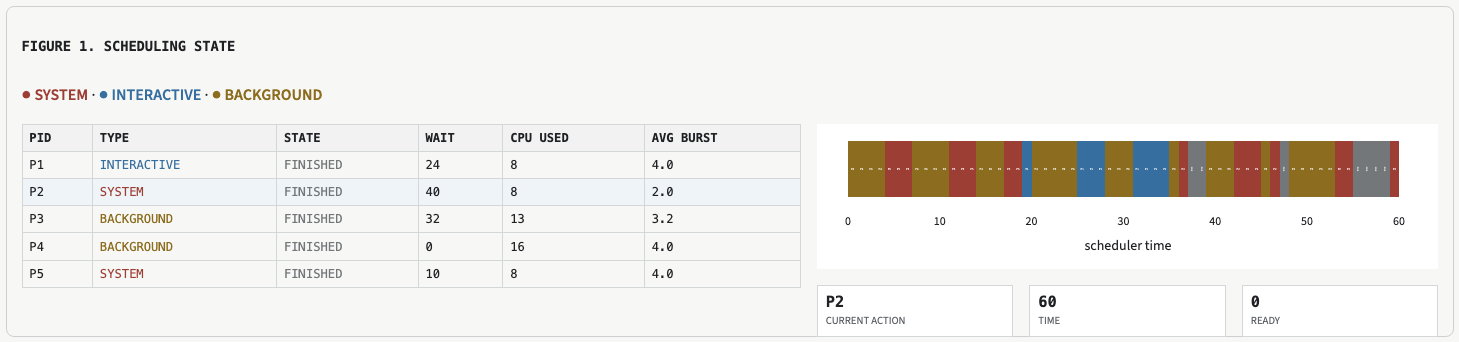
\includegraphics[width=\columnwidth]{figures/fig_scheduling_state.png}
  \caption{Dashboard view of \method{} on seed 42 with 5 processes.
           Left: per-process scheduling state.  Right: Gantt timeline
           spanning 60 ticks.  P2 (SYSTEM) accumulates the highest
           waiting time due to repeated I/O blocking; P4 (BACKGROUND)
           receives priority upon exceeding the aging threshold.}
  \label{fig:frontend1}
\end{figure}

\begin{figure}[t]
  \centering
  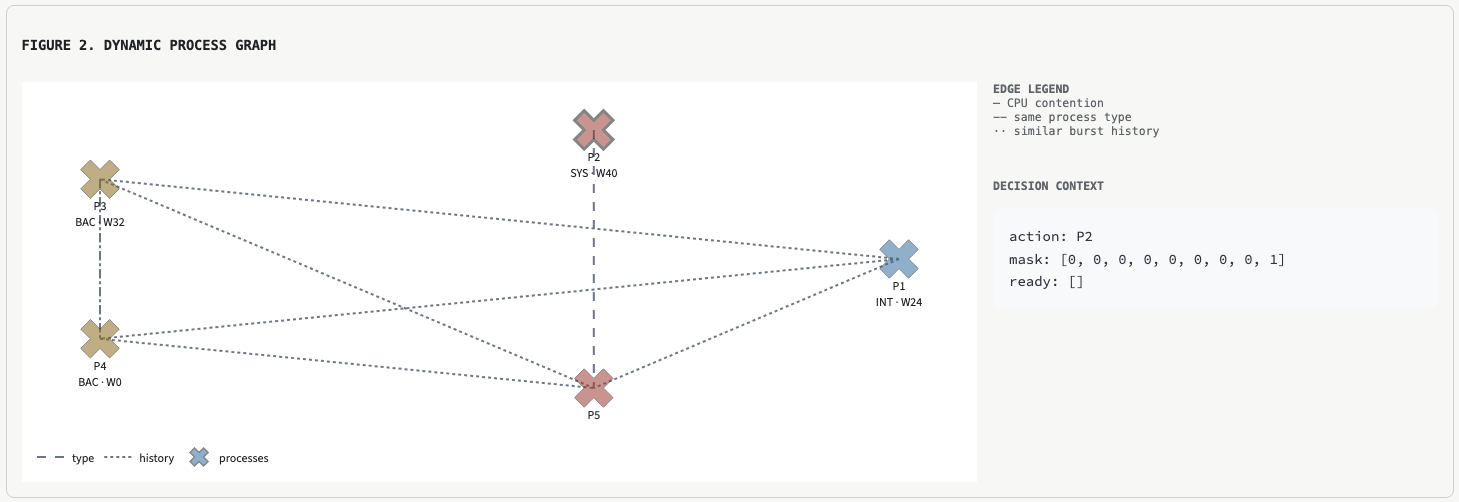
\includegraphics[width=\columnwidth]{figures/fig_process_graph.png}
  \caption{Dynamic process graph as rendered in the dashboard.  Three
           edge families are shown: CPU contention (solid), type
           similarity (dashed), and burst-history similarity (dotted).
           The graph is reconstructed at every tick and aggregated by
           GraphSAGE into a 48-dimensional policy input.}
  \label{fig:frontend2}
\end{figure}

\begin{figure}[tp]
  \centering
  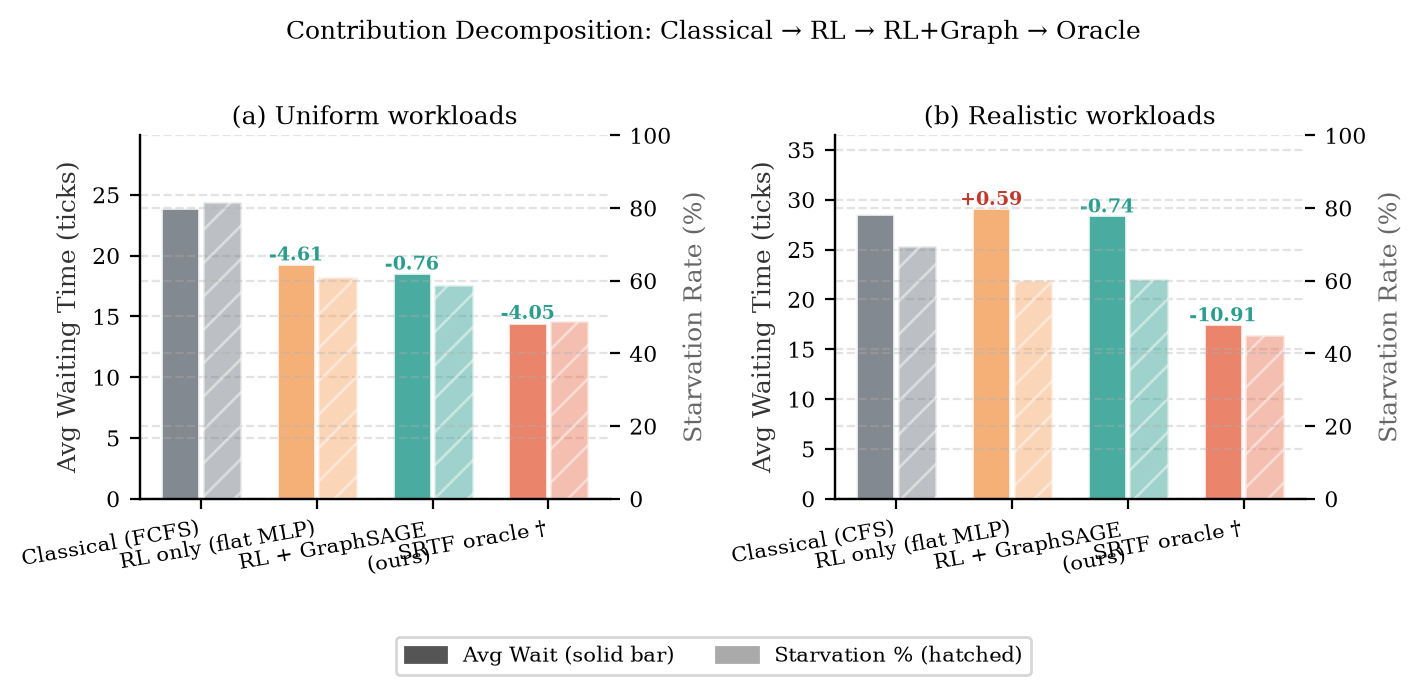
\includegraphics[width=\columnwidth]{figures/fig_contribution_decomp.png}
  \caption{Contribution decomposition
           (Classical $\to$ RL $\to$ RL+Graph $\to$ SRTF).
           Solid bars: average waiting time.  Hatched bars: starvation
           rate.  On realistic workloads, RL alone does not significantly
           outperform CFS ($+0.6$, n.s.), but the addition of the graph
           yields a significant improvement ($-0.7$).}
  \label{fig:decomp}
\end{figure}

% =====================================================================================
\section{Discussion}
\label{sec:discuss}

CFS proves to be a highly competitive baseline on realistic workloads.
Its virtual-runtime weighting effectively handles heterogeneous
exponential-burst processes, leaving minimal room for a flat-MLP policy
to improve upon.  The graph representation addresses this limitation by
providing relational context.  Through burst-history similarity edges,
the policy identifies clusters of processes exhibiting similar
behaviour, using this information as an approximate proxy for which
processes will complete quickly.  This constitutes a learned
approximation of SRTF-style reasoning, derived entirely from observable
history rather than hidden future information.

The remaining 10.91-tick gap to SRTF on realistic workloads is
attributable primarily to an information-theoretic barrier.  Exponential
distributions exhibit a coefficient of variation of exactly 1.0; the
next burst may differ from the historical average by several multiples.
No causal policy---one that cannot observe future burst lengths---can
recover this information.  On uniform workloads, where variance is
substantially lower, this gap narrows to 4.05 ticks.

The starvation reduction of 12--24 percentage points over CFS represents
the most consistent finding across all experimental conditions.  CFS
contains no starvation threshold; the aging penalty
(Eq.~\ref{eq:reward}) provides the policy with a strong gradient to
attend to long-waiting processes.  To the best of our knowledge, this is
the first RL-based scheduler that acquires anti-starvation behaviour
purely through reward shaping.

\subsection{Limitations}

All experiments are conducted in a Python-based simulator; no kernel
integration has been performed.  The current implementation is limited
to 8 concurrent processes due to the fixed observation size.  The
``realistic'' workloads are generated from textbook distributions rather
than captured from production \texttt{/proc} traces.  Additionally, all
three edge types employ the same mean-pooling aggregation;
relation-specific aggregation kernels such as
R-GCN~\cite{rgcn} may yield further improvements.

% =====================================================================================
\section{Conclusion}
\label{sec:conclusion}

This paper presents \method{}, a graph-structured reinforcement learning
framework for CPU process scheduling that jointly optimises efficiency
and fairness.  Two principal findings emerge.  First, the soft-priority
aging reward consistently reduces starvation by 12--24 percentage points
relative to CFS and all classical baselines across every experimental
condition.  Second, the graph representation is essential: on realistic
workloads---those most representative of production OS
environments---a flat RL agent cannot significantly outperform CFS.  The
relational structure encoded by the dynamic process graph provides the
signal necessary to identify scheduling opportunities that a flat
observation vector misses.

Future work will focus on eBPF~\cite{ebpf} integration for deployment
within a real Linux kernel, extension to variable-length process queues
via sparse graph attention mechanisms, and evaluation on production
workload traces.

% =====================================================================================
\bibliographystyle{IEEEtran}
\bibliography{references}

\end{document}
